\chapter{背景} \label{chap::background}
本章首先简要介绍深度学习和深度神经网络的基本原理,以及基于深度学习的现代目标检测算法。之后介绍现代深度学习普遍面临的存储、运算开销问题,以及随之兴起的高效深度学习的进展。最后介绍本文重点关注的神经网络量化压缩加速技术近年来在算法、软件及硬件方面的发展,面临的主要挑战,以及与后续章节讨论内容相关的其他工作。

深度学习是机器学习的子集,深度学习使用神经网络学习并解决一系列机器学习问题~\citep{lecun2015deep}。神经网络由一系列\emph{神经元}及神经元之间的\emph{连接}构成。\emph{神经元}是神经网络的基本感知单元,神经元根据其在神经网络拓扑中的位置被划归至不同\emph{层}。第一层神经元被称为网络输入,最后一层神经元被称为网络输出。每一神经元有各自的数值表示,其数值大小表示该感知单元对网络输入的响应强度。网络输入之后的神经网络每一层内,神经元与前一层部分或全部神经元相\emph{连接},且同一层内的神经元互不连接。每一连接有表示其连接强度的数值大小,同一神经网络内表示所有连接强度的数值组成的集合称为该模型的\emph{参数}。一般认为层数超过 8 层的神经网络为“深度”神经网络~\citep{krizhevsky2012imagenet}。

深度神经网络通过\emph{前向传播}和\emph{反向传播}在目标任务上进行推理和梯度计算,使用\emph{随机梯度下降}等算法对模型参数进行更新。以常见的有监督机器学习任务为例:在某一完整标注的数据集 $\mathcal{D} = \{x_i, y_i\}_{i=1\ldots N}$ 上,欲训练一包含参数 $\mathcal{W} = \{w_1, \ldots w_L\}$ 的 $L$ 层神经网络 $\FpNet$。首先需要以一定方法对模型参数 $\mathcal{W}$ 进行\emph{初始化},得到模型每一层在训练步数 $t=0$ 时的参数 $\{w_1^{t=0}, \ldots w_L^{t=0}\}$。随后采样一批量大小为 $B$ 的小批量数据 $\{x_j, y_j\}_{j=1\ldots B} \in \mathcal{D}$,按照一定流程 $p(\cdot)$ 将 $[x_{1, \ldots B}]$ 做预处理后,作为网络输入送入模型 $\FpNet$ 中,表示为 $a_0 = p(x_{1, \ldots B})$。之后从模型第 $l=1$ 层开始,根据当前层的参数 $w_l^t$ 计算层内各神经元的响应值 $\tilde{a}_{l, k}, k = 1, \ldots K_l$,其中 $K_l$ 表示当前层神经元数目。$\tilde{a}_{l, k}$ 被计算为与该神经元相连接的上一层神经元的响应数值与连接强度的乘积加和——以全连接网络为例,$\tilde{a}_l = w_l^t a_{l-1}$。每一神经元在实际更新其激活值前,还要先经过特定非线性函数 $g(\cdot)$,以增加网络的表达能力——即每一神经元的实际激活值被计算为 $a_{l, k} = g(\tilde{a}_{l, k})$。根据此过程从网络第 $1$ 层计算至网络第 $L$ 层,得到模型的最终输出 $a_L = \FpNet(a_0)$。上述过程即为模型的前向传播,又称为模型的\emph{推理}。

神经网络的输出 $a_L$ 在不同任务中,以不同方式被解释。例如在分类任务中,$a_L \in \mathbb{R}^{B \times C}$ 中的元素 $a_{L, b, c}$ 表示小批量中第 $b$ 个样本属于第 $c$ 类物体的概率;在回归任务中,$a_L \in \mathbb{R}^{B \times T}$ 中的元素 $a_{L, b, t}$ 表示第 $b$ 个样本在第 $t$ 个回归任务上的输出值。\footnote{注意此处 $a_{L, b, t}$ 的下标 $t$ (指代模型\emph{任务 task})与参数 $w_l^t$ 的上标 $t$ (指代训练的\emph{步数 time stamp})不一致,请读者根据上下文区分。}在模型训练过程中,前向传播过程结束后,需要根据学习任务定义的损失函数 $\mathcal{L}$ 和当前小批量输入的标注 $[y_{1, \ldots B}]$ 计算模型在 $t=0$ 步的\emph{损失}值 $\mathcal{L}(a_L, y_{1, \ldots B})$,并根据\emph{链式法则}计算模型参数的梯度 $\{\mathrm{d}w_1, \ldots \mathrm{d}w_L\}$。同样以全连接网络为例,在模型第 $l$ 层神经元对应的梯度 $\mathrm{d} a_l$ 计算就绪后,该层连接参数的梯度被计算为 $\mathrm{d} w_l = \mathrm{d} a_l \diff{g(\tilde{a}_l)}{\tilde{a}_l} a_{l-1}$。从网络第 $L$ 层开始,从后向前通过链式法则计算梯度 $\mathrm{d}w_L, \ldots \mathrm{d}w_1$ 至网络第 $1$ 层的过程即被称为模型的反向传播。

在模型反向传播完成后,则通过梯度下降等方法,从参数梯度的相反方向更新模型参数。也就是说,神经网络的训练一般使用一阶方法。模型参数更新的实际幅度与参数梯度成正比,梯度幅度与实际更新步长间的比值称为\emph{学习率}。具体地,在给定学习率 $\alpha$ 后,模型参数基本的梯度下降更新表示为 $w_l^{t+1} := w_l^t - \alpha \mathrm{d} w_l$。参数更新至 $w_{1, \ldots L}^{t+1}$ 之后,继续下一轮迭代。随机采样小批量数据直至训练集 $\mathcal{D}$ 耗尽的过程称为训练 1 \emph{轮},参数较多或数据集较为复杂的任务可能要训练数百轮,最终输出收敛后的模型 $f_{\mathcal{W}^*}$。

深度学习算法非常简明,但正是这些简单参数化操作的非线性组合,在近年来爆发增长的可用数据及计算力加持下,逐渐印证了 \emph{more is different}~\citep{anderson1972more} 的哲学原理——深度学习在计算机视觉、自然语言处理、推荐系统等方面取得了显著成功:在计算机视觉领域,深度学习被应用于语义分割~\citep{yuan2019object}、物体分类~\citep{xie2019self}、物体检测~\citep{liu2019cbnet}、图像生成~\citep{song2019generative}、姿态检测~\citep{bulat2020toward} 等任务;在自然语言处理领域,深度学习被应用于机器翻译~\citep{edunov2018understanding}、语言模型~\citep{shoeybi2019megatron}、提问--回答~\citep{zhang2020retrospective}、语义分析~\citep{raffel2019exploring}、文本生成~\citep{guo2018long} 等任务;在其他传统和新兴领域,深度学习还被应用于医学图像分割~\citep{ronneberger2015u}、药物研发~\citep{alperstein2019all}、强化学习~\citep{mnih2015human}、迁移学习~\citep{wang2019easy}、推荐系统~\citep{rendle2019difficulty}、点击率预测~\citep{deng2020sparse} 等任务。
% ==============================================================================
%  Object Detection in Deep Learning Era
% ==============================================================================
\section{基于深度学习的目标检测}
目标检测是计算机视觉中最基本且重要的任务之一。给定一张输入图片,目标检测算法需要给出图片中目标物体边界框(bounding box)的精确坐标,并给出每一边界框对应的目标类别。因此,目标检测算法需要同时完成针对输入图片的回归和分类任务。在深度学习被应用到计算机视觉任务之前,目标检测算法一般依赖领域专家手工设计的图像特征提取算子,以及滑动窗口、多尺度级联、目标结构化拆分等准确度改进手段。这一阶段的代表性工作包括 Viola Jones 检测算法~\citep{viola2001rapid, viola2004robust}、HOG 检测算法(Histogram of Oriented Gradients, \citet{dalal2005histograms})、DPM 检测算法(Deformable Part-based Model, \citet{felzenszwalb2008discriminatively, felzenszwalb2009object, girshick2011object, girshick2012rigid})等。

由于深度神经网络——特别是深度卷积神经网络——在适当的模型结构及损失函数设计下,能够有效地提取图像的空间、语意特征,并能够有效学习分类、回归等任务,因此近年来被广泛运用于目标检测任务中。下文称基于深度学习的目标检测算法为\emph{现代目标检测算法}。现代目标检测算法肇始于 RCNN~\citep{girshick2015region},之后逐渐发展分化为\emph{二阶段检测算法(two-stage detectors)}和\emph{一阶段检测算法(one-stage detectors)}。
% ------------------------------------------------------------------------------
%    Two-stage detectors
% ------------------------------------------------------------------------------
\subsection{二阶段检测算法}
二阶段检测算法的核心思路是:将目标检测拆分为两部分,算法第一阶段算法先提出一定数目的候选边界框,通过一定方法过滤明显错误的候选框后,算法第二阶段再对保留的候选框做细粒度修正和分类,最终达到输出准确度。算法第一阶段一般称为 proposal,第二阶段一般称为 refinement,其遵循的是“由粗到细”(from coarse to fine)的设计思想。本节介绍近年来有代表性的二阶检测算法。

\begin{figure}[htb]
  \centering
  \includegraphics[width=0.8\columnwidth]{Img/Background/RCNN.pdf}
  \caption{RCNN 的算法架构,图片来自~\citet{girshick2015region}}
  \label{img::background::RCNN}
\end{figure}

RCNN (Regions with CNN features, \citet{girshick2015region})是最先使用深度卷积网络的现代目标检测算法。其架构如图~\ref{img::background::RCNN} 所示,首先在输入图片上使用 selective search~\citep{van2011segmentation} 选取一定数目的候选检测框(region of interests,下文简称 RoI)并裁剪得到子图,随后使用深度卷积网络在缩放至特定尺寸的子图上提取图片特征,最后使用 SVM 在图片特征上对候选框内容分类,以及后续的检测框坐标回归等任务。RCNN 算法在 Pascal VOC07 目标检测挑战~\citep{Everingham10} 上达到了 $58.5\%$ 平均准确度(mean average precision,下文简称 mAP),但其选取候选框的流程较为耗时,且在每一候选区域内分别提取特征的做法造成了大量重复冗余,因此 RCNN 算法的运行速度较慢(单张图片检测时长约 14 秒)。

\begin{figure}[htb]
  \centering
  \includegraphics[width=0.6\columnwidth]{Img/Background/spm.pdf}
  \caption{SPPNet 的算法架构,图片来自~\citet{he2015spatial}}
  \label{img::background::SPPNet}
\end{figure}

针对 RCNN 存在的特征提取冗余问题,\citet{he2015spatial} 提出了针对图片的空间金字塔采样操作(spatial pyramid pooling layer),可以在不同尺寸的输入图片或子图上生成等长的特征表示(图~\ref{img::background::SPPNet})。借助于 SPP 算子,每张图片可以在检测模型训练前一次性完成特征采样,之后检测子区域的特征可从该等长全局特征上生成,从而避免了 RCNN 中重复提取图片特征的缺点。SPPNet 在 Pascal VOC07 上达到了 $59.2\%$ mAP,然而其主要问题是不能在均一的训练流程内同时训练 SPP 层和用于检测输出的全连接层,导致了可能的模型表达能力受限。

\begin{figure}[htb]
  \centering
  \includegraphics[width=0.7\columnwidth, trim=0 20em 18em 0, clip]{Img/Background/fast_RCNN.pdf}
  \caption{Fast RCNN 的算法架构,图片来自~\citet{girshick2015fast}}
  \label{img::background::fast_RCNN}
\end{figure}

Fast RCNN~\citep{girshick2015fast} 使用深度全卷积网络在输入图片上直接提取全图特征,随后在各 RoI 对应的特征区域使用 RoI pooling 操作提取等长的 RoI 特征(图~\ref{img::background::fast_RCNN})。由于 RoI pooling 完全可导,加之 Fast RCNN 使用 Multi-task loss 将各任务子网络的训练规整至同一训练框架下,解决了 RCNN 和 SPPNet 算法各阶段参数需要分离训练的问题。Fast RCNN 在 Pascal VOC07 上达到了 $70.0\%$ mAP,但其运行速度仍然受限于 RoI 生成算法。

\begin{figure}[htb]
  \centering
  \begin{subfigure}[t]{0.35\columnwidth}
    \centering
    \includegraphics[width=\columnwidth]{Img/Background/faster_RCNN.pdf}
    \caption{Faster RCNN 的算法架构}
    \label{img::background::faster_rcnn_arch}
  \end{subfigure}
  \quad
  \begin{subfigure}[t]{0.6\columnwidth}
    \centering
    \includegraphics[width=\columnwidth, trim=0 0 13em 0, clip]{Img/Background/rpn.pdf}
    \caption{RPN 模型结构及预定义 anchor boxes}
    \label{img::background::faster_rcnn_rpn}
  \end{subfigure}
  \caption{Faster RCNN 的算法架构~\subref{img::background::faster_rcnn_arch}及 RPN~\subref{img::background::faster_rcnn_rpn},图片来自~\citet{ren2015faster}}
  \label{img::background::faster_rcnn}
\end{figure}

为加快 RoI 候选生成速率,Faster RCNN~\citep{ren2015faster} 提出了 region proposal network (RPN)直接在主干卷积网络的输出特征上生成候选 RoI (图~\ref{img::background::faster_rcnn_rpn})。具体地,RPN 在卷积特征每一空间位置按照预先定义的一系列不同尺寸和长宽比的锚框(anchor boxes)通过分类和回归子网络,生成一系列包含表示候选框内容为前景目标的\emph{目标性(objectness)}指标的候选 RoI,再将其送入 Faster RCNN 的 RoI pooling 框架中进行后续计算(图~\ref{img::background::faster_rcnn_arch})。由于 RPN 完全可导,使得 Faster RCNN 成为第一个能够完全端到端训练的二阶目标检测算法。Faster RCNN 在 Pascal VOC07 上达到 $73.2\%$ mAP,在 MS COCO~\citep{lin2014microsoft} 上达到 $21.9\%$ mAP。后续工作 RFCN~\citep{dai2016r}、Light-head RCNN~\citep{li2017light} 等在 Faster RCNN 框架内进一步减少了运算开销。

\begin{figure}[htb]
  \centering
  \includegraphics[width=0.4\columnwidth]{Img/Background/FPN.pdf}
  \caption{FPN 的算法架构,图片来自~\citet{lin2017feature}}
  \label{img::background::FPN}
\end{figure}

Feature pyramid networks~\citep{lin2017feature} 是对二阶检测算法主干网络特征提取的加强(图~\ref{img::background::FPN})。一般认为深度卷积网络深层特征空间信息不足而语意信息丰富,浅层特征空间信息精确而语意信息缺乏。FPN 从主干网络不同深度提取特征,并通过上采样操作将深层特征放大叠加至浅层特征中,从而得到同时包含精确空间信息和丰富语意信息的图片特征。FPN 在 MS COCO 上达到了 $36.2\%$ mAP。
% ------------------------------------------------------------------------------
%    One-stage detectors
% ------------------------------------------------------------------------------
\subsection{一阶段检测算法}
二阶段检测算法能带来较高的检测精度,且第一阶段的后处理可以在二阶段检测子模型中避免简单负样本过多导致难样本产生的梯度被噪声掩盖的问题。然而二阶段检测算法所需的计算量较大,会影响模型运行的实时性,因此注重模型端到端运行速度的一阶段检测算法应运而生。一阶段检测算法使用同一网络完成候选框分类、回归任务,直接输出最终结果。本节介绍近年来有代表性的一阶段检测算法。

\begin{figure}[htb]
  \centering
  \includegraphics[width=0.4\columnwidth]{Img/Background/YOLO_bbox.pdf}
  \caption{YOLOv2 所用的边界框回归算法,图片来自~\citet{redmon2017yolo9000}}
  \label{img::background::yolo_bbox}
\end{figure}

YOLO~\citep{redmon2016you} 是第一个使用深度卷积网络的一阶目标检测算法。YOLO 是 you only look once 的缩写,即该算法仅使用单一网络对输入图片进行区域划分,并计算每一区域上检测框的位置和类别(图~\ref{img::background::yolo_bbox}),从而在保证 Pascal VOC07 上 $52.7\%$ mAP 的同时达到了 155 FPS 的运行效率。后续工作~\citet{redmon2017yolo9000, redmon2018yolov3} 进一步改进了 YOLO 的检测准确度和运行效率。

\begin{figure}[htb]
  \centering
  \includegraphics[width=0.8\columnwidth]{Img/Background/ssd.pdf}
  \caption{SSD 的算法架构,图片来自~\citet{liu2016ssd}}
  \label{img::background::ssd}
\end{figure}

SSD~\citep{liu2016ssd} 是 Single Shot MultiBox Detector 的缩写。SSD 在主干网络不同深度提取不同尺寸的图片特征,并在特征每一位置分别计算与不同尺寸及长宽比的预定义锚框间的回归误差及分类置信度(图~\ref{img::background::ssd})。由于使用了多尺度特征,其检测准确度相较 YOLO 获得了显著提升。在运行速率达到 59 FPS 同时,能够在 Pascal VOC07 上达到 $76.8\%$ mAP。

\begin{figure}[htb]
  \centering
  \begin{subfigure}[t]{0.65\columnwidth}
    \includegraphics[width=\columnwidth]{Img/Background/retinanet.pdf}
    \caption{RetinaNet 模型架构}
    \label{img::background::retina_net}
  \end{subfigure}
  \quad
  \begin{subfigure}[t]{0.3\columnwidth}
    \includegraphics[width=\columnwidth]{Img/Background/focal_loss.pdf}
    \caption{RetinaNet 所用的 Focal loss}
    \label{img::background::focal_loss}
  \end{subfigure}
  \caption{RetinaNet~\subref{img::background::retina_net} 及其使用的分类损失函数 Focal loss~\subref{img::background::focal_loss},图片来自~\citet{lin2017focal}}
  \label{img::background::retinanet_focalloss}
\end{figure}

\citet{lin2017focal} 指出一阶段检测器准确度较二阶段检测器低的关键原因是训练过程中存在过多简单负样本,导致参数梯度被大量简单样本产生的噪声掩盖,而二阶段检测器由于 RPN 之后会通过非极大抑制(non-maximum suppression,下文简称 NMS)滤掉大量低置信度样本而不存在此问题。因此 \citet{lin2017focal} 通过减小分类交叉熵损失中简单样本的权重以避免生成过多梯度噪声,这种改进的损失函数即为 focal loss (图~\ref{img::background::focal_loss})。在此基础上训练的 RetinaNet (图~\ref{img::background::retina_net})是目前准确度最高的一阶段检测器之一,在 MS COCO 上达到了 $39.1\%$ mAP。
% ==============================================================================
%  Efficient Deep Learning
% ==============================================================================
\section{高效深度学习}
Batch normalization~\citep{ioffe2015batch}、残差连接~\citep{He_2016}、大批量分布式训练~\citep{goyal2017accurate} 等技术的出现,使得我们能够在大量数据上训练深度超过 1000 层的超大型模型~\citep{He_2016}。数据量和模型容量的提升显著改进了深度学习的准确度,但也导致了其训练和部署过程开销愈发巨大。以使用 ResNet-101 主干网络且包含 FPN 的 Faster RCNN 目标检测模型为例:在 16 块 GPU 上进行分布式训练时,每次基于 all-reduce 的同步需要在集群内传输 14.52GB 梯度信息;在模型部署时需占用 60.52MB 内存,在常用的尺寸为 $1280 \times 800$ 像素的输入下,执行一次前向推理的运算量达到了 283.14G FLOPS。为降低深度学习模型的部署和训练开销,高效深度学习近年来成为了工业界和学术界的研究热点之一。本节从深度学习模型的高效结构设计、高效训练方法和高效部署方法三个维度介绍该领域的进展。
% ------------------------------------------------------------------------------
%    Efficient architectures
% ------------------------------------------------------------------------------
\subsection{高效模型结构设计}
设计参数量和运行计算量都较少的轻量级网络模型对深度学习的训练、部署过程都有帮助:在训练过程中,较少的参数量使得分布式训练所需同步的梯度量等比例减小;在部署过程中,较小的参数量可减少运行时设备访存和缓存上下文交换,较少的运行计算量可提高模型实时性。更重要的是,轻量级网络的部署并不对部署平台的存储、运算单元有特殊需求,可部署至任意支持神经网络运行的平台上。本节介绍近年来有代表性的轻量级网络模型。

\begin{figure}[htb]
  \centering
  \includegraphics[width=0.5\columnwidth]{Img/Background/fire_module.pdf}
  \caption{SqueezeNet 所用的 Fire module 模块,图片来自~\citet{iandola2016squeezenet}}
  \label{img::background::fire_module}
\end{figure}

SqueezeNet~\citep{iandola2016squeezenet} 是第一个在 ImageNet~\citep{krizhevsky2012imagenet} 这一大规模分类任务上达到 AlexNet~\citep{krizhevsky2012imagenet} 级别准确度的轻量模型。SqueezeNet 主要使用图~\ref{img::background::fire_module} 所示的 Fire module 减小模型参数及运算量:Fire module 首先通过 $1\times 1$ 卷积减少特征通道数,之后通过混合的 $1\times 1$、$3\times 3$ 卷积提取并扩充特征。SqueezeNet 将模型参数量从 AlexNet 的 240MB 减少至 4.8MB,同时在 ImageNet 上达到了 $57.5\%$ 的 Top-1准确度。

\begin{figure}[htb]
  \centering
  \begin{subfigure}[t]{0.4\columnwidth}
    \centering
    \includegraphics[width=\columnwidth]{Img/Background/separable_conv.pdf}
    \caption{通道分离卷积}
    \label{img::background::separable_conv}
  \end{subfigure}
  \quad
  \begin{subfigure}[t]{0.5\columnwidth}
    \centering
    \includegraphics[width=\columnwidth]{Img/Background/expansion_conv.pdf}
    \caption{通道扩展分离卷积}
    \label{img::background::expansion_conv}
  \end{subfigure}
  \caption{MobileNet 所用的通道分离卷积~\subref{img::background::separable_conv} 和 MobileNet-v2 所用的通道扩展分离卷积~\subref{img::background::expansion_conv},图片来自~\citet{Sandler_2018}}
  \label{img::background::mobile_nets}
\end{figure}

MobileNet~\citep{howard2017mobilenets} 是针对移动平台部署环境设计的轻量化网络。MobileNet 使用通道分离卷积(depth-wise separable convolution),不同于采样所有输入通道的常规 2D 卷积核,通道分离卷积每一卷积核仅采样输入的一个通道,且各卷积核对输入通道的采样不重叠,从而使模型卷积层参数数量和计算量都减少了 $C_{\mathrm{in}}$ 数量级(图~\ref{img::background::separable_conv})。MobileNet 参数量减少至 4.2MB,在 ImageNet 上 Top-1 准确度为 $70.6\%$。后续工作 MobileNet-v2~\citep{Sandler_2018} 使用反向 bottleneck 结构(图~\ref{img::background::expansion_conv}),在 $3\times 3$ 通道分离卷积前使用 $1\times 1$ 卷积扩展特征通道数以增强模型表现力,参数量为 3.4MB 情况下在 ImageNet 上达到 $72.0\%$ 准确度。MobileNet-v3~\citep{howard2019searching} 使用模型自动搜索技术~\citep{zoph2018learning} 进一步改善了模型的准确度/运算开销,标准通道数的 MobileNet-v3 参数量进一步减少至 2.5MB,在 ImageNet 上达到 $67.4\%$ 的 Top-1 准确度。

\begin{figure}[htb]
  \centering
  \begin{subfigure}[t]{0.45\columnwidth}
    \centering
    \includegraphics[width=\columnwidth]{Img/Background/channelshuffle.pdf}
    \caption{通道混合操作}
    \label{img::background::channel_shuffle}
  \end{subfigure}
  \quad
  \begin{subfigure}[t]{0.45\columnwidth}
    \centering
    \includegraphics[width=\columnwidth]{Img/Background/shufflenet_unit.pdf}
    \caption{ShuffleNet 组成单元}
    \label{img::background::shufflenet_unit}
  \end{subfigure}
  \caption{ShuffleNet 所用的通道混合操作~\subref{img::background::channel_shuffle} 和基本组成单元~\subref{img::background::shufflenet_unit},图片来自~\citet{zhang2018shufflenet}}
  \label{img::background::shuffle_net}
\end{figure}

ShuffleNet~\citep{zhang2018shufflenet} 使用分组卷积减少模型参数和计算量,并通过组间通道混合保持模型的表达能力。如图~\ref{img::background::channel_shuffle} 所示,ShuffleNet 将模型特征分为多组,计算量较大的 $3\times 3$ 卷积仅在同组通道内进行;同时在 $1 \times 1$ 卷积之后设置通道混合操作在各组间传递特征信息(图~\ref{img::background::shufflenet_unit}),以保证模型的表达能力。标准通道数的 ShuffleNet 针对 $224\times 224$ 尺寸输入的推理运算开销为 140M FLOPS,在 ImageNet 上 Top-1 准确度为 $67.6\%$。

\begin{figure}[htb]
  \centering
  \begin{subfigure}[t]{0.35\columnwidth}
    \centering
    \includegraphics[width=\columnwidth]{Img/Background/MnasNet_overallflow.pdf}
    \caption{MnasNet 平台相关模型搜索流程}
    \label{img::background::mnasnet_overall_flow}
  \end{subfigure}
  \quad
  \begin{subfigure}[t]{0.6\columnwidth}
    \centering
    \includegraphics[width=\columnwidth]{Img/Background/MnasNet_searchspace.pdf}
    \caption{MnasNet 搜索空间}
    \label{img::background::mnasnet_search_space}
  \end{subfigure}
  \caption{MnasNet 以部署平台实际推理耗时作为搜索反馈~\subref{img::background::mnasnet_overall_flow},并使用了层次化搜索空间~\subref{img::background::mnasnet_search_space}。图片来自~\citet{tan2019mnasnet}}
  \label{img::background::mnasnet}
\end{figure}

近两年来模型自动化搜索技术~\citep{zoph2018learning, liu2018darts, lu2019nsga} 在许多场景上超过了先前手工设计的模型,因此也被应用到了轻量化模型设计上。MnasNet~\citep{tan2019mnasnet} 以强化学习搜索方式为基础,将模型在目标平台上实际推理耗时作为搜索反馈的一部分(图~\ref{img::background::mnasnet_overall_flow}),并设计了部署至低算力设备的层次化搜索空间(图~\ref{img::background::mnasnet_search_space})。在 Pixel 1 手机上,使用 CPU 运行的 MnasNet 能够以 78ms 的单样本实际推理耗时在 ImageNet 上达到 $75.2\%$ Top-1 准确度。

\begin{figure}[htb]
  \centering
  \includegraphics[width=0.7\columnwidth]{Img/Background/fbnet_flow.pdf}
  \caption{FBNet 的搜索算法架构,图片来自~\citet{wu2019fbnet}}
  \label{img::background::fbnet}
\end{figure}

FBNet~\citep{wu2019fbnet} 是基于随机超网络和可微分搜索的另一个注重部署平台推理性能的轻量化模型搜索工作。如图~\ref{img::background::fbnet} 所示,FBNet 将包含所有候选操作的搜索空间组成一个超网络,并在其上做随机参数化采样,采样的概率参数通过 Gumbel Softmax~\citep{jang2016categorical, maddison2016concrete} 在搜索训练过程中可导。同时在搜索前对所有候选操作在部署平台上测速,并通过查找表将被采样结构的推理延迟加入到搜索过程损失函数中。部署至 Samsung Galaxy S8 手机后,以 CPU 运行的 FBNet 能够以 19.8ms 的单样本实际推理耗时在 ImageNet 上达到 $73.0\%$ Top-1 准确度。

\begin{figure}[htb]
  \centering
  \includegraphics[width=0.75\columnwidth]{Img/Background/scalecompare.pdf}
  \caption{EfficientNet 在搜索时对候选模型通道数、深度、特征图分辨率做同一缩放,图片来自~\citet{tan2019efficientnet}}
  \label{img::background::efficient_net}
\end{figure}

EfficientNet~\citep{tan2019efficientnet} 是目前轻量化模型中在准确度/运行开销间权衡最为出色的工作之一。EfficientNet 同样基于强化学习搜索算法~\citep{zoph2018learning},但引入了一个关键发现——高准确度模型在其通道数、深度、特征图分辨率统一向上或向下缩放后,相较分离缩放搜索的模型更容易保持较高准确度——从而极大地减少了搜索空间。EfficientNet-B0 模型能在 5.3MB 参数量、0.39G FLOPS 推理计算量下,在 ImageNet 上达到 $76.3\%$ Top-1 准确度。
% ------------------------------------------------------------------------------
%    Efficient training
% ------------------------------------------------------------------------------
\subsection{高效模型训练方法}
除设计搜索轻量模型外,还有大量正交于模型结构的高效训练方法。深度神经网络的模型训练相较于模型推理,其额外的开销在于梯度的反向传播计算,以及分布式训练场景下各节点间梯度同步。本节分别介绍近年来针对训练过程中对于梯度反传和梯度同步的代表性加速方法。

\begin{figure}[htb]
  \centering
  \begin{subfigure}[t]{0.45\columnwidth}
    \centering
    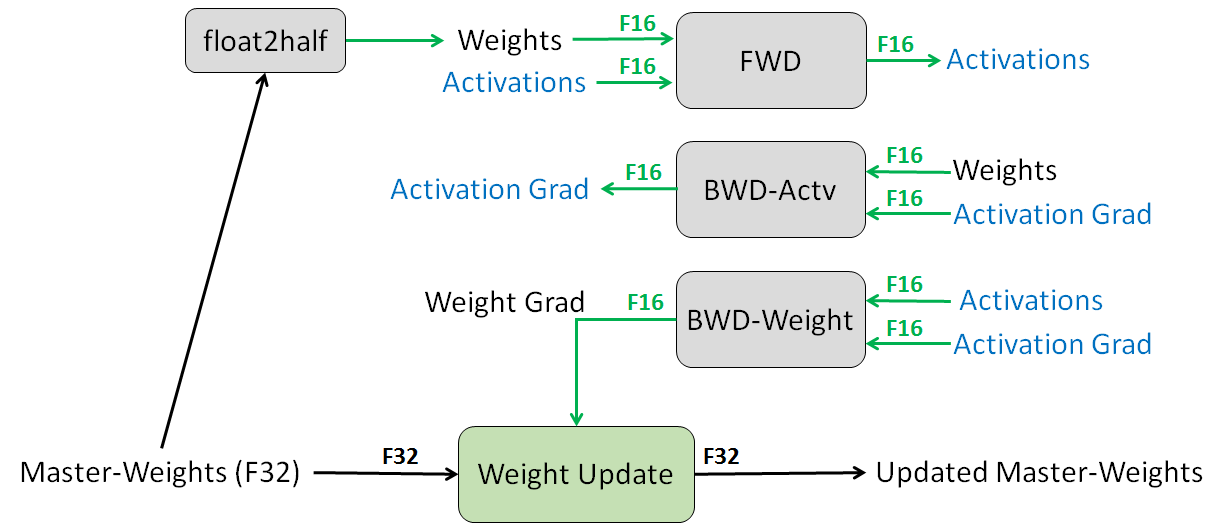
\includegraphics[width=\columnwidth]{Img/Background/mixed_prec_iteration.png}
    \caption{FP16 训练流程}
    \label{img::background::fp16_ops}
  \end{subfigure}
  \quad
  \begin{subfigure}[t]{0.45\columnwidth}
    \centering
    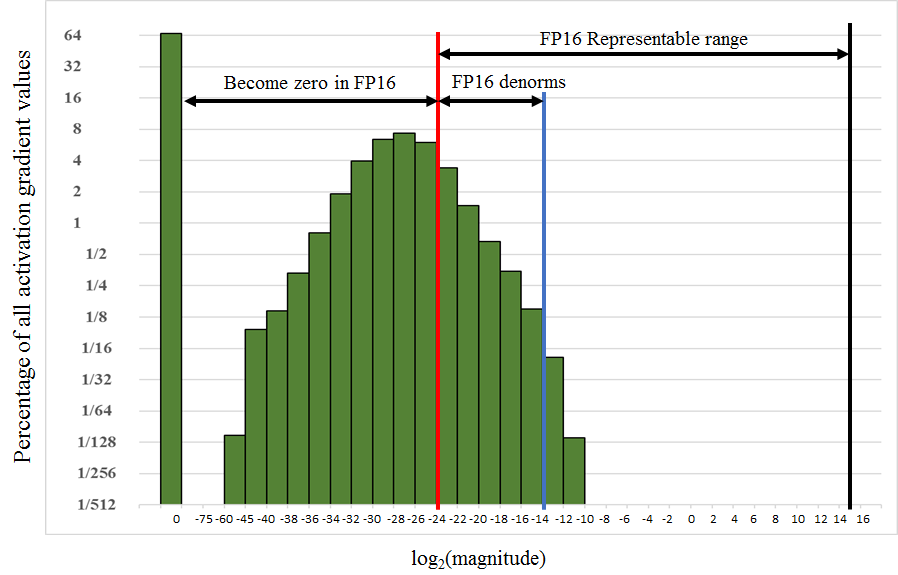
\includegraphics[width=\columnwidth]{Img/Background/ssd_ag_log_histo_coarse.png}
    \caption{梯度分布与 FP16 数值范围}
    \label{img::background::fp16_grads}
  \end{subfigure}
  \caption{模型训练时使用 FP16 精度进行前向反向计算,并将梯度缩放后更新底层的 FP32 精度模型参数~\subref{img::background::fp16_ops}。FP16 数值精度有限,需在反传开始前缩放 loss 值以确保梯度计算不会出现数值截断~\subref{img::background::fp16_grads}。图片来自~\citet{micikevicius2018mixed}}
  \label{img::background::fp16_training}
\end{figure}

深度神经网络一般使用单精度浮点存储模型参数和进行数值计算,\citet{micikevicius2018mixed} 指出使用半精度浮点(FP16)也可在不影响模型准确度的前提下将大部分用于不同任务的深度神经网络训练至收敛。FP16 训练流程如图~\ref{img::background::fp16_ops} 所示,在前向传播过程中,模型参数和输入激活被截断转换至 FP16,之后通过 FP16 数值逻辑计算得出输出激活;在反向传播过程中,以 FP16 表示的梯度与以 FP16 缓存的前向过程临时变量通过 FP16 数值逻辑计算得出模型参数和输入激活的梯度,并继续以链式法则进行反向传播。模型参数梯度就绪后,转换至 FP32 格式对实际保存的 FP32 模型参数进行更新。注意如图~\ref{img::background::fp16_grads} 所示,由于 FP16 数值范围有限,幅度值较小的梯度在计算时可能会下溢为 0,因此需要在反向传播开始前适当缩放损失函数值 $\mathcal{L}$,使反向传播中所有梯度保持在 FP16 数值范围内;在将梯度转换至 FP32 时,再将梯度范围缩放至原有数值。

在大部分现代 GPU 及其他包含浮点计算单元的硬件上,同一设备的 FP16 算力一般是 FP32 算力的一倍以上。例如 NVIDIA RTX 2080Ti GPU 的 FP32 算力为 13.45T FLOPS,而其 FP16 算力高达 26.90T FLOPS \citep{nvidia2018turing}。除~\citet{micikevicius2018mixed} 外,\citet{abadi2016tensorflow, dean2012large} 也报告了使用 FP16 或 BFLOAT16 数值精度进行深度神经网络训练的结果。在实际应用中,FP16 一般能将模型训练时间缩短一倍左右。

\begin{figure}[htb]
  \centering
  \includegraphics[width=0.75\columnwidth]{Img/Background/int8_training.pdf}
  \caption{INT8 训练对前向过程和反向过程的修改,图片来自~\citet{zhu2019towards}}
  \label{img::background::int8_training}
\end{figure}

另一个更激进的方法是将网络前向、后向传播中的参数、激活量化至带缩放因子的整数张量,从而将模型训练中计算量的大部分替换为整数数值逻辑(图~\ref{img::background::int8_training})。例如,\citet{das2018mixed} 报告了使用 INT16 数值精度训练深度卷积网络,可在不损失模型准确度的情况下获得 $1.8\times$ 训练吞吐量提升;\citet{zhu2019towards} 通过调整量化函数截断阈值和修改模型训练策略,可以在 INT8 数值精度下将 MobileNet~\citep{howard2017mobilenets, Sandler_2018} 系列模型训练收敛,且在 NVIDIA GTX 1080Ti GPU 上实际达到 $+22\%$ 的训练速度提升。

针对分布式训练中各节点间梯度同步问题,目前主要有两种加速方案。一种是使用梯度稀疏化、梯度量化、梯度信息编码等方式减少节点间的通讯量。例如 \citet{wen2017terngrad} 将节点间梯度三值化为 $\{-1, 0, 1\}$,并在不超过 $2\%$ 准确度损失的情况下将 GoogLeNet~\citep{szegedy2015going} 训练至收敛;\citet{aji2017sparse, lin2018deep} 通过幅度阈值对通讯梯度做稀疏化,\citet{lin2018deep} 报告了将 ResNet-50 训练梯度从 97MB 压缩至 0.35MB 而不损失模型准确度。另一种是利用反向传播逐层计算的特性,在模型计算某一层梯度时,同步以就绪的其他梯度,以实现“隐藏”通信时间的效果。\citet{abadi2016tensorflow, paszke2019pytorch} 利用 CUDA stream 异步执行的特性,将 NCCL~\citep{jeaugey2017nccl} 的通信原语与 cuDNN~\citep{chetlur2014cudnn} 的计算操作按调用顺序传递至训练 GPU 的 CUDA stream 中,从而实现对通信开销的隐藏。\citet{peng2019generic} 通过对神经网络不同层间通信的优先级调度以及根据集群网络环境对通信算法参数的优化,在 Parameter Server~\citep{li2014scaling}、基于 all-reduce 的同步训练等分布式训练范式上均获得了显著加速。
% ------------------------------------------------------------------------------
%    Efficient deployment
% ------------------------------------------------------------------------------
\subsection{高效模型部署方法}
神经网络模型在部署时主要面临的挑战仍然是其过高的存储和推理计算开销。为减轻算法模型对计算资源的需求,提高计算资源的利用率,高效模型部署技术的发展主要分为两个方向:从\emph{算法}层面减少部署模型的存储和推理复杂度,从\emph{系统}层面根据部署环境优化模型推理运行时对计算资源的利用率。

\begin{figure}[htb]
  \centering
  \includegraphics[width=0.75\columnwidth]{Img/Background/deep_compression.pdf}
  \caption{DeepCompression 部署流程,图片来自~\citet{han2015deep}}
  \label{img::background::deep_compression}
\end{figure}

近年来从算法层面提升模型部署运行效率的工作,几乎都可以归类至 \citet{han2015deep, han2017efficient} 提出的 DeepCompression 框架内(图~\ref{img::background::deep_compression})。DeepCompression 对模型部署的优化加速包含三个流程:通过\emph{剪枝}(pruning)技术减少模型参数量,通过\emph{量化}(quantization)技术降低模型参数和激活数值位宽,最后通过其他无损压缩技术进一步减小模型部署后的体积。剪枝技术主要包括:
{
  \setlist[enumerate]{}
  \begin{enumerate*}[1)]
    \item 非结构化剪枝~\citep{han2015learning},即通过一定标准将模型中参数值置为 $0$ 而提高模型稀疏度,在支持稀疏操作的专有硬件上可降低能耗、提高推理效率;
    \item 结构化剪枝~\citep{li2016pruning},即删除模型卷积层中的部分卷积核和全连接层中的部分通道,可直接地减小模型的存储和计算复杂度;
    \item 层级剪枝~\citep{chen2018shallowing},直接删除网络模型中的部分冗余层。
  \end{enumerate*}
}
模型部署时的量化技术主要包括:
{
  \setlist[enumerate]{}
  \begin{enumerate*}[1)]
    \item 将模型参数量化或二值化至低比特表示~\citep{courbariaux2015binaryconnect, hou2018loss},从而减少模型部署后体积;
    \item 将模型参数和激活同时量化至低比特~\citep{rastegari2016xnor, jacob2018quantization},从而利用整数数值逻辑加速模型部署后的推理过程。
  \end{enumerate*}
}
DeepCompression 流程最后一步使用 Huffman 编码~\citep{van1976construction} 进一步减小模型体积。其他压缩加速算法还包括模型参数的低秩分解~\citep{sainath2013low}、高效矩阵乘法~\citep{lavin2016fast} 等。

\begin{figure}[htb]
  \centering
  \includegraphics[width=0.75\columnwidth]{Img/Background/tvm_stack.pdf}
  \caption{TVM 部署系统架构,图片来自~\citet{chen2018tvm}}
  \label{img::background::tvm}
\end{figure}

TODO
% ==============================================================================
%  Quantized Neural Networks: Algorithms, Softwares and Hardwares
% ==============================================================================
\section{量化神经网络}
量化神经网络~\citep{guo2018survey} 及其特例二值化神经网络~\citep{qin2020binary} 通过将神经网络模型参数、激活、梯度使用特定方法压缩至低比特定点数、整数,或根据某一查找表进行映射至离散值(例如根据数值符号和阈值映射至 $\{-1, 0, 1\}$ ),达到减少模型参数体积(量化模型参数)、加速模型运算(同时量化模型参数和激活)及减少模型分布式训练通信量(量化模型梯度)的目的。具体地,给定一待量化输入 $x\in \mathbb{R}$,量化函数 $Q(\cdot)$ 将其映射至一离散集合 $\mathbb{T}$ 中的对应值,即 $\hat{x} = Q(x): \mathbb{R} \to \mathbb{T}$;在反向传播阶段,则根据相应的求导原则 $\diff{\hat{x}}{x}$ 将上游梯度 $\diff{\mathcal{L}}{\hat{x}}$ 传递至 $x$ 以继续梯度的链式法则计算。近年来量化神经网络领域大量工作主要集中探讨两个话题:量化函数 $Q(\cdot)$ 的设计方式,以及在给定量化函数后对量化模型 $\QuantNet$ 的优化方法。本节将依次介绍量化函数设计和量化函数优化方面的代表性工作。最后,本节还将介绍用于训练部署量化神经网络的软件和硬件实现。
% ------------------------------------------------------------------------------
%    Quantizers
% ------------------------------------------------------------------------------
% ○ Quantizers
%   § BinaryConnect
%   § BNN
%   § XNOR-Net
%   § DoReFa
%   § HWGQ
%   § PACT
%   § ABC-Net
%   § LQ-Nets
%   § APoT
% ○ Training methods
%   § QAT
%     □ Integer-only
%     □ Distillation Quantization / Apprentice
%     □ Loss-aware binary/ternary
%     □ LR-Nets / Probabilistic BNN
%     □ LIQ
%     □ DSQ
%   § Post-training methods
%     □ WhitePaper
%     □ Few-data calibration
%     □ Data-free / same but different
%   § Allocate the bit budget
%     □ AutoML methods (HWQ)
%     □ Metric-based methods (Hessian aware quant)
\subsection{量化函数设计}
BinaryConnect~\citep{courbariaux2015binaryconnect} 是最早使用量化技术减少模型参数体积的工作。在前向传播时,BinaryConnect 根据模型参数 $w$ 的幅度大小,\emph{随机地}将其映射至 $\{-1, 1\}$;在反向传播过程中,使用 Straight Though Estimator (\citet{bengio2013estimating},下文简称 STE) 将量化函数的上游梯度直接复制至全精度输入。为防止模型参数由于前向过程中幅度信息 $|w|$ 丢失而造成过多偏移,每步参数更新会将参数范围限制在 $[-1, 1]$ 之间。具体地,
\begin{align}
  \text{\textbf{Forward}: } & \hat{w} = 
    \begin{cases}
      1 & \text{ with probability } p = \hat{\sigma}(w) \\
      -1 & \text{ with probability } 1 - p
    \end{cases} \\
  \text{\textbf{Backward}: } & \diff{\mathcal{L}}{w} = \diff{\mathcal{L}}{\hat{w}} \label{eq::background::ste}
\end{align}
其中 $\diff{\mathcal{L}}{\hat{w}}$ 为损失函数 $\mathcal{L}$ 传导至 $\hat{w}$ 处的梯度,$\hat{\sigma}(w) = \max(0, \min(\frac{w+1}{2}, 1))$。在使用 $\diff{\mathcal{L}}{w}$ 更新 $w$ 后,再将 $w$ 范围限制在 $[-1, 1]$ 之间。

Binarized Neural Networks (\citet{hubara2016binarized}, 下文简称 BNN) 进一步将模型激活也映射至 $\{-1, 1\}$,以便使用\emph{算术位移}操作完成模型的前向传播。为减轻模型前向传播的计算开销,BNN 使用确定性量化处理模型激活:
\begin{align}
  \text{\textbf{Forward}: } & \hat{x} = 
    \begin{cases} 
      1 & \text{ if } x \ge 0 \\
      -1 & \text{ otherwise}
    \end{cases}
    \label{eq::background::sign}
\end{align}
同时 BNN 也提出了使用算术位移实现的 Batch normalization~\citep{ioffe2015batch} 和 AdaMax~\citep{kingma2014adam},并报告上述基于位移的实现在 GPU 上可节省 $60\%$ 的模型推理时间。

为进一步提高量化参数 $\hat{w}$ 针对全精度参数 $w$ 的近似准确性,XNOR-Net \citep{rastegari2016xnor} 为量化参数引入了浮点缩放 $\alpha$,并将量化过程视为针对量化后参数和缩放的最小二乘问题:
\begin{align}
\arg\min_{\hat{w}, \alpha} &= \| \alpha\hat{w} - w \|_2 \label{eq::background::xnor_opt}
\end{align}
\eqref{eq::background::xnor_opt} 存在闭式解 $\alpha^* = \frac{\|w\|_1}{n}$,$\hat{w}^* = \sign(w)$,其中 $n$ 为参数张量 $w$ 中所含元素个数,$\sign$ 即为 \eqref{eq::background::sign}。

值得注意的是,在 BNN 和 XNOR-Net 中,量化后的激活 $\hat{x}$ 和参数 $\hat{w}$ 满足 $\hat{x}, \hat{w} \in \{-1, 1\}$,因此它们之间的点积操作可用异或(XNOR)及 1-位计数(bitcount)完成:
\begin{align}
  \hat{x} \cdot \hat{w} &= N - 2 \cdot \mathrm{bitcount}(\mathrm{xnor}(\hat{x}, \hat{w})) \label{eq::background::xnor_dot}
\end{align}
其中 $N$ 为向量 $\hat{w}, \hat{x}$ 中所含元素个数。

DoReFa-Net~\citep{zhou2016dorefanet} 引入了 k-bit 量化函数 $Q_k(\cdot)$,使得量化点集 $\mathbb{T}$ 中可用元素数目达到了 $2^k-1$。具体地,给定一全精度输入 $x\in [0, 1]$,k-bit 量化函数定义为:
\begin{align}
  \text{\textbf{Forward}: } & \hat{x} = \frac{\lfloor (2^k - 1)x \rceil}{2^k - 1} \label{eq::background::dorefa_fwd} \\
  \text{\textbf{Backward}: } & \diff{\mathcal{L}}{x} = \diff{\mathcal{L}}{\hat{x}}
\end{align}
其中 $\Round{\cdot}$ 为舍入操作符。对于模型参数 $w$,DoReFa-Net 使用 $\tanh$ 函数将其映射至 $[-1, 1]$,再线性映射至 $Q_k(\cdot)$ 的定义域内;对于经过非线性层后的模型激活 $x$,则直接将其截断至 $[0, 1]$;对于梯度 $g$ 的处理方式和 $w$ 类似,但是会在量化前叠加幅度范围在 $\pm \frac{|g|}{2}$ 之内的均匀噪声。

Half Wave Gaussian Quant (\citet{cai2017deep},下文简称 HWGQ)注意到非线性层之后的模型激活 $x$ 通常符合从 0 截断的半波高斯分布,故使用分段式函数定义 $Q(\cdot)$。在给定量化位宽 $k$ 之后,
\begin{align}
  \text{\textbf{Forward}: } & \hat{x} = 
    \begin{cases} 
      q_i & \text{ if } x \in (t_i, t_{i+1}] \\
      0 & \text{ } x \le 0
    \end{cases}
    \label{eq::background::hwgq}
\end{align}
其中 $\{q_1, \ldots q_{2^k-1}\}$ 为量化点集,$t_0=0, t_1, \ldots, t_{2^k-1}, t_{2^k}=\infty$ 为分段函数的边界。$\{q_i, t_j\}, i, j \in {1, \ldots 2^k-1}$ 的取值通过 Lloyd~\citep{lloyd1982least} 算法求解优化问题
\begin{align}
  \arg\min_{q_i, t_j} \|\hat{x} - x\|_2
\end{align}
得出。

PArameterized Clipping acTivation (\citet{choi2018pact} 下文简称 PACT),为减少模型激活量化误差,设计了带可学习上界参数 $\beta$ 的线性截断函数代替 ReLU,并将截断后的激活值线性缩放至 $[0, 1]$ 之后传入 \eqref{eq::background::dorefa_fwd} 中。在模型反向传播过程中,$\beta$ 使用接收到的梯度进行更新。 

DoReFa-Net 和 PACT 所用的 k-bit 线性均匀量化函数 \eqref{eq::background::dorefa_fwd} 实际是将量化后的 $\hat{x}$ 表示为其编码向量 $b_x = [b_1, \ldots b_k], b_i \in \{0, 1\}$ 与 2-幂基底 $v^{(2)} = [2^0, 2^1, \ldots 2^{k-1}]$ 和缩放因子 $\alpha$ 的点积,即 $\hat{x} = \alpha v^{(2)} b_x^T$。LQ-Nets~\citep{Zhang_2018} 指出量化函数所用基底可以不一定是 2-幂基底 $v^{(2)}$,而可以在训练过程中学习适合目标网络数值特性的基底 $v = [v_1, \ldots, v_k], v_i \in \mathbb{R}$。由基底 $v$ 同样可以在 k-bit 编码上生成 $2^k$ 个量化点 $[q_1, \ldots, q_{2^k}]$,其中 $q_1 = v [0, \ldots 0]^T, q_{2^k} = v [1, \ldots 1]^T$。具体地,LQ-Nets 所用量化函数 $\hat{x} = Q_{\mathrm{LQ}}(x, v)$ 实现为
\begin{align}
  \text{\textbf{Forward}: } & \hat{x} = v b_x^T \label{eq::background::lq_fwd}
\end{align}
其中 $b_x$ 为 $q_i \le x < q_{i+1}$ 时 $i$ 对应的编码向量。使用 \eqref{eq::background::lq_fwd} 对实数向量点积 $wa^T, w, a \in \mathbb{R}^N$ 操作数量化后,点积操作可以用 \eqref{eq::background::xnor_dot} 在 $w, a$ 的编码向量上完成,即
\begin{align}
  Q_{\mathrm{LQ}}(w, v^{(w)}) Q_{\mathrm{LQ}}(a, v^{(a)})^T &= \sum_{i=1}^{k_w} \sum_{j=1}^{k_a} v^{(w)}_i v^{(a)}_{j} (b^{(w)}_i b^{(a)}_j)
\end{align}
其中 $k_w, k_a$ 分别为操作数 $w, a$ 的量化位宽,$v^{(w)} \in \mathbb{R}^{k_w}, v^{(a)} \in \mathbb{R}^{k_a}$ 为 $w, a$ 在 LQ-Nets 量化模式中的基底,$b^{(w)}, b^{(a)}$ 间的点积可以由 \eqref{eq::background::xnor_dot} 完成。

\begin{figure}[htb]
  \centering
  \includegraphics[width=\columnwidth]{Img/Background/APoT.pdf}
  \caption{在 $[0, 1]$ 范围内,APoT 量化方式(右)与均匀量化(左)和 2-幂量化(中)的对比。图片来自 \citet{li2019additive}}
  \label{img::background::apot}
\end{figure}

Additive Power-of-Two (\citet{li2019additive},下文简称 APoT)将量化位宽 $k$ 拆分为 $n$ 个位宽为 $m$ 的 2-幂量化子项,将输入编码为 $n$ 个子项的加和,以避免普通 2-幂量化的量化点过于集中在零点附近的问题。具体地,在给定实数输入 $x\in [0, \alpha)$ 后,其量化函数 $\hat{x} = Q_{\mathrm{APoT}}(x; \alpha, m, n)$ 实现为:
\begin{align}
  Q_{\mathrm{APoT}}(x; \alpha, m, n) &= \gamma \times \{ \sum_{i=0}^{n-1} p_i \} \\
  \text{where } p_i &\in \{0, \frac{1}{2^i}, \frac{1}{2^{i+n}}, \ldots \frac{1}{2^{i + 2^{m-1}n}}\} \notag
\end{align}
其中 $\gamma$ 为缩放因子,确保 $Q_{\mathrm{APoT}}(x; \alpha, m, n)$ 输出的最大项数值为 $\alpha$,各项位宽 $m$ 和项数 $n$ 满足 $k = mn$。在 $\alpha = 1, m = n = 2$ 时,APoT 量化方式与其他常见量化方式的对比见图~\ref{img::background::apot}。
% ------------------------------------------------------------------------------
%    Training methods
% ------------------------------------------------------------------------------
\subsection{量化模型优化方法}
一般神经网络模型在量化后会遭受准确度损失,因此需要使用特定方法恢复量化模型的准确度。目前量化模型的优化方法主要分两类:需要在特定数据集上进行前向传播和反向传播计算,使用得到的梯度更新模型参数的\emph{量化感知训练}(\emph{Quantization-aware Training},下文简称 QAT)方法;以及不需要反向传播计算,在使用少量数据或完全没有训练数据情况下,进行模型量化参数标定及其他操作即可完成转换部署的\emph{量化后处理}(\emph{Post-training Quantization},下文简称 PTQ)方法。

\begin{figure}[htb]
  \centering
  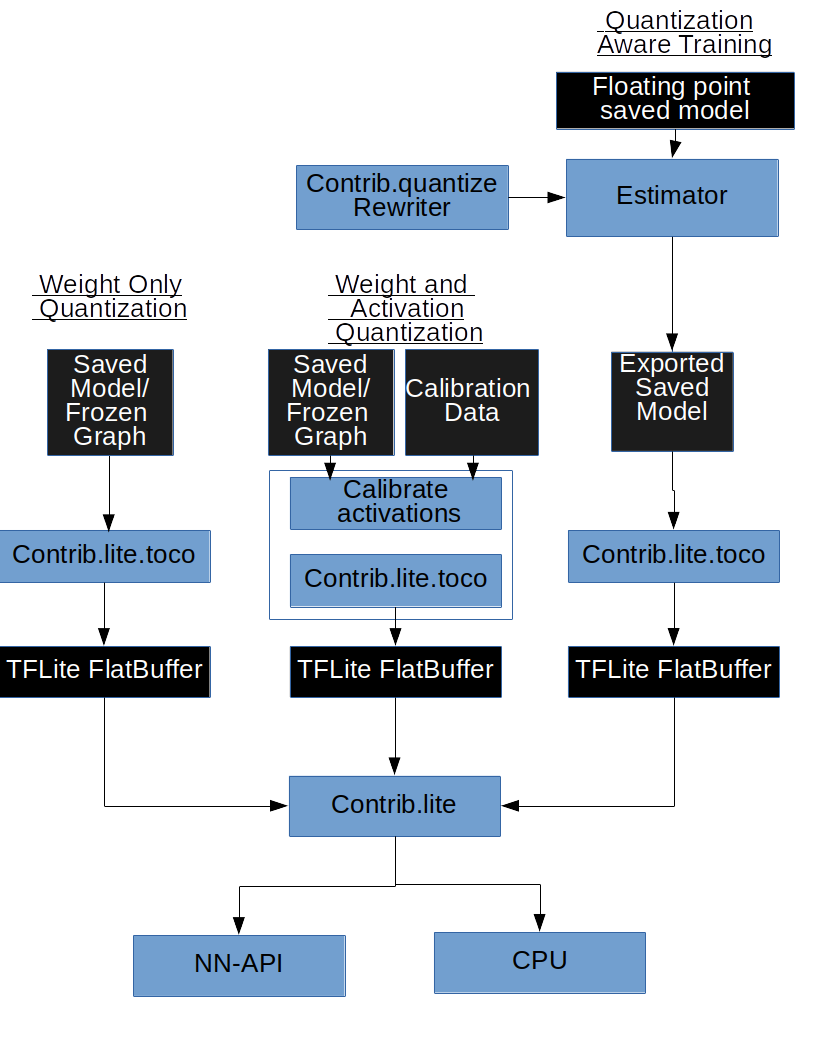
\includegraphics[width=0.75\columnwidth]{Img/Background/qat_ptq.png}
  \caption{TensorFlow Lite 中模型参数量化(左)、量化后处理方法(中)和量化感知训练方法(右)的算法流程。图片来自~\citet{krishnamoorthi2018quantizing}}
  \label{img::background::qat_ptq}
\end{figure}

PTQ 方法包含对模型激活的标定,对模型正则化参数的调整,以及在不使用梯度信息的情况下对模型参数进行微调。由于各类量化函数运行前需获知被量化输入的数值范围,故对神经网络模型参数、激活同时量化时,需要确定模型各层激活数值范围,即对模型激活进行\emph{标定}。TensorFlow Lite 的 PTQ 模块~\citep{abadi2016tensorflow, krishnamoorthi2018quantizing} 在标定数据集上运行待量化的模型,记录模型中每层参数的最大最小值,并通过动量 $M$ 以指数移动平均(Exponential Moving Average)方式更新每层激活的量化范围(图~\ref{img::background::qat_ptq} 中间部分流程)。\citet{he2018learning, peters2018probabilistic} 指出原模型中 BN 等正则化层的统计参数并不能有效地匹配量化模型的激活分布,因此提出在标定数据集上运行量化后的模型时,应根据量化激活的分布情况重新统计并更新模型中的正则化参数。在无法接触到训练数据或标定数据的情况下,\citet{nagel2019data, meller2019same} 通过调整量化模型参数分布,在不改变模型输入——输出映射关系的前提下减少模型量化误差,恢复量化模型准确度。

QAT 方法与一般神经网络训练方法类似,将量化后的模型在训练集上进行前向传播和反向传播计算,并按照特定策略对模型参数进行梯度下降更新(图~\ref{img::background::qat_ptq} 右侧流程)。QAT 方法的主要问题是量化函数对于量化输入并不可导,各类工作针对此问题提供了不同的解决方案:模型量化的早期工作 \citet{courbariaux2015binaryconnect, hubara2016binarized, rastegari2016xnor, zhou2016dorefanet} 使用 STE~\eqref{eq::background::ste} 将量化函数输出接受的梯度直接复制至其输入,以确保链式法则能继续进行。由于量函数的全精度输入与求导时所用的量化输出数值并不一定相同,所以使用 STE 反传梯度会出现梯度不匹配问题,且在量化数值精度较低时更为明显。为解决此问题,\citet{cai2017deep} 探索了 HWGQ 量化函数的可微分导数近似;\citet{louizos2018relaxed} 使用可微分的 Gumbel Softmax~\citep{jang2016categorical, maddison2016concrete} 算子,在全精度模型的训练过程中逐渐将模型参数和激活由连续分布“硬化”至离散分布;\citet{gong2019differentiable} 提出的 Differentiable soft quantization 算子将分段函数的导数使用可微分的类 $\tanh$ 函数近似,并在训练过程中逐渐接近实际分段函数。除改进 STE 的梯度准确度外,其他实现高精度 QAT 的方法包括:\citet{peters2018probabilistic, shayer2018learning} 将神经网络的量化操作视为随机过程,即量化后的参数或激活服从特定的参数化离散分布,在反向传播时即可针对分布参数求导;\citet{hou2016loss, hou2018loss} 利用 Adam 优化算法~\citep{kingma2014adam} 中的二阶动量信息,使用拟牛顿法直接对模型量化权重的缩放因子 $\alpha_w$ 和量化表示 $b_w$ 求导并优化;\citet{polino2018model, mishra2018apprentice} 使用知识蒸馏技术~\citep{hinton2015distilling} 将高准确度大模型的输出作为“软标签”引入 QAT 过程,以改善量化模型的准确度;\citet{jung2019learning} 使用参数化的量化函数,并在 QAT 阶段将量化函数参数引入模型任务损失计算,以此通过模型反向传播时的梯度优化量化函数。
% ------------------------------------------------------------------------------
%    Softwares and hardwares
% ------------------------------------------------------------------------------
\subsection{相关软硬件实现}
TODO
